\documentclass{UCF_ETD}
% \usepackage{times} % obsolete font package
\usepackage{url,hyperref,lineno,microtype,subcaption}
\usepackage{datetime, fmtcount, etoolbox, fcprefix}
\usepackage[T1]{fontenc}
\usepackage[utf8]{inputenc}
\usepackage{mathptmx}
\usepackage{graphicx}
\usepackage{amsmath,amssymb,amsfonts}
\usepackage{algorithmic}
\usepackage{textcomp}
\usepackage{cite}
\usepackage{graphics}
\usepackage{color,soul}
\usepackage{multirow,makecell}
\usepackage{pdfpages}
% \usepackage[backend=biber,style=numeric]{biblatex}    
% %Use absolute paths to .bib-files for the subfiles to understand their location:
\usepackage{float}
\usepackage{chapterbib}
\usepackage{subfiles}
\newcommand{\ignore}[1]{}
\newcommand{\tss}[1]{\textsuperscript{#1}}
\renewcommand{\ul}{}
\newcommand{\tsu}[1]{\textsubscript{#1}}
\newcommand{\td}{\textasciitilde}



\title{\uppercase{Corticomuscular adaptation to mechanical perturbations in a seated locomotor task}} %Must be typed in all caps.
\author{\uppercase{Seyed Yahya Shirazi}} % typed in all caps



\prevdegreeii{B.Sc. AmirKabir University of Technology (Tehran Polytechnic), 2011}
\prevdegreei{M.Sc. AmirKabir University of Technology (Tehran Polytechnic), 2014}
% commands available for 
% \prevdegreei{ }
% \prevdegreeii{ }
% \prevdegreeiii{ }

\thesisname{dissertation}
% \thesisname prints out document type. Replace bracket text with dissertation for Ph.D students

\degreename{Doctor of Philosophy in Mechanical Engineering}
% type out degree name here.

\departmentsname{Mechanical and Aerospace Engineering}
% replace with department name if applicable.  Otherwise, do not include.

%\schoolname{Kenneth G. Dixon School of Accounting}
% replace with school name if applicable.  Otherwise, do not include.

\collegename{Engineering and Computer Science}
% replace with college name

\termname{Spring}
% replace with semester

\termyear{2021}
% replace with year. Term year is also used to generate copyright year.

\advisorname{Helen J. Huang}
% replace with Major Professor if applicable.  Otherwise, do not include.


\begin{document}

\frontmatter
% applies roman numerals as page numbers

\maketitle
% prints out school info as named above

\copyrightpage{~Seyed Yahya Shirazi}
% includes copyright symbol. Term year is automatically inserted before the author name.  Replace the author name with your own, but keep the tilde in place. 

\begin{abstract}
Seated locomotor tasks such as cycling or recumbent stepping improve walking performance during rehabilitation. Cortical control during walking is most pronounced when the person is perturbed. But, the electrocortical dynamics during perturbed seated tasks has not been studied in detail. The primary purpose of this research was to quantify cortical and muscular responses to mechanical perturbations during recumbent stepping. We also aimed to quantify possible differences between young and older adults' responses to perturbed stepping. Seventeen young adults and eleven older adutls completed four perturbed arms and leg stepping tasks. We perturbed the stepping with brief 200ms increased movement resistance using a controllable serovmotr on our recumbent stepper. We asked subjects to step smoothly, use both arms and legs and follow the visual pacing cue set at 60 steps per minute. We used high-density electroencephalogrphy (EEG) with 128 electrodes to record brain activity, 16 electromyography (EMG) sensors to record muscle actvitty, and stepping kinematics using the servomotor's encoder. 
% abstract files can be added here.  I recommend using \input over \include
\end{abstract}

\dedication{Dedicated to my love, Maryam.}
% creates vertically and horizontally centered dedication page.  If larger than a paragraph, remove the \vspace*fil commands from the dedication section in the class file.

\begin{acknowledgments}
The acknowledgments page is optional. If you choose to use it, it should appear after the Abstract, but before the Table of Contents.
\end{acknowledgments}

\tableofcontents

\listoffigures

\listoftables

\mainmatter
% restarts page numbering with arabic numbers

\subfileinclude{chapters/chap0}

\subfileinclude{chapters/chap1}

\subfileinclude{chapters/chap2}

\subfileinclude{chapters/chap3}

\appendix

\chapter{IRB DOCUMENTS}
\newpage
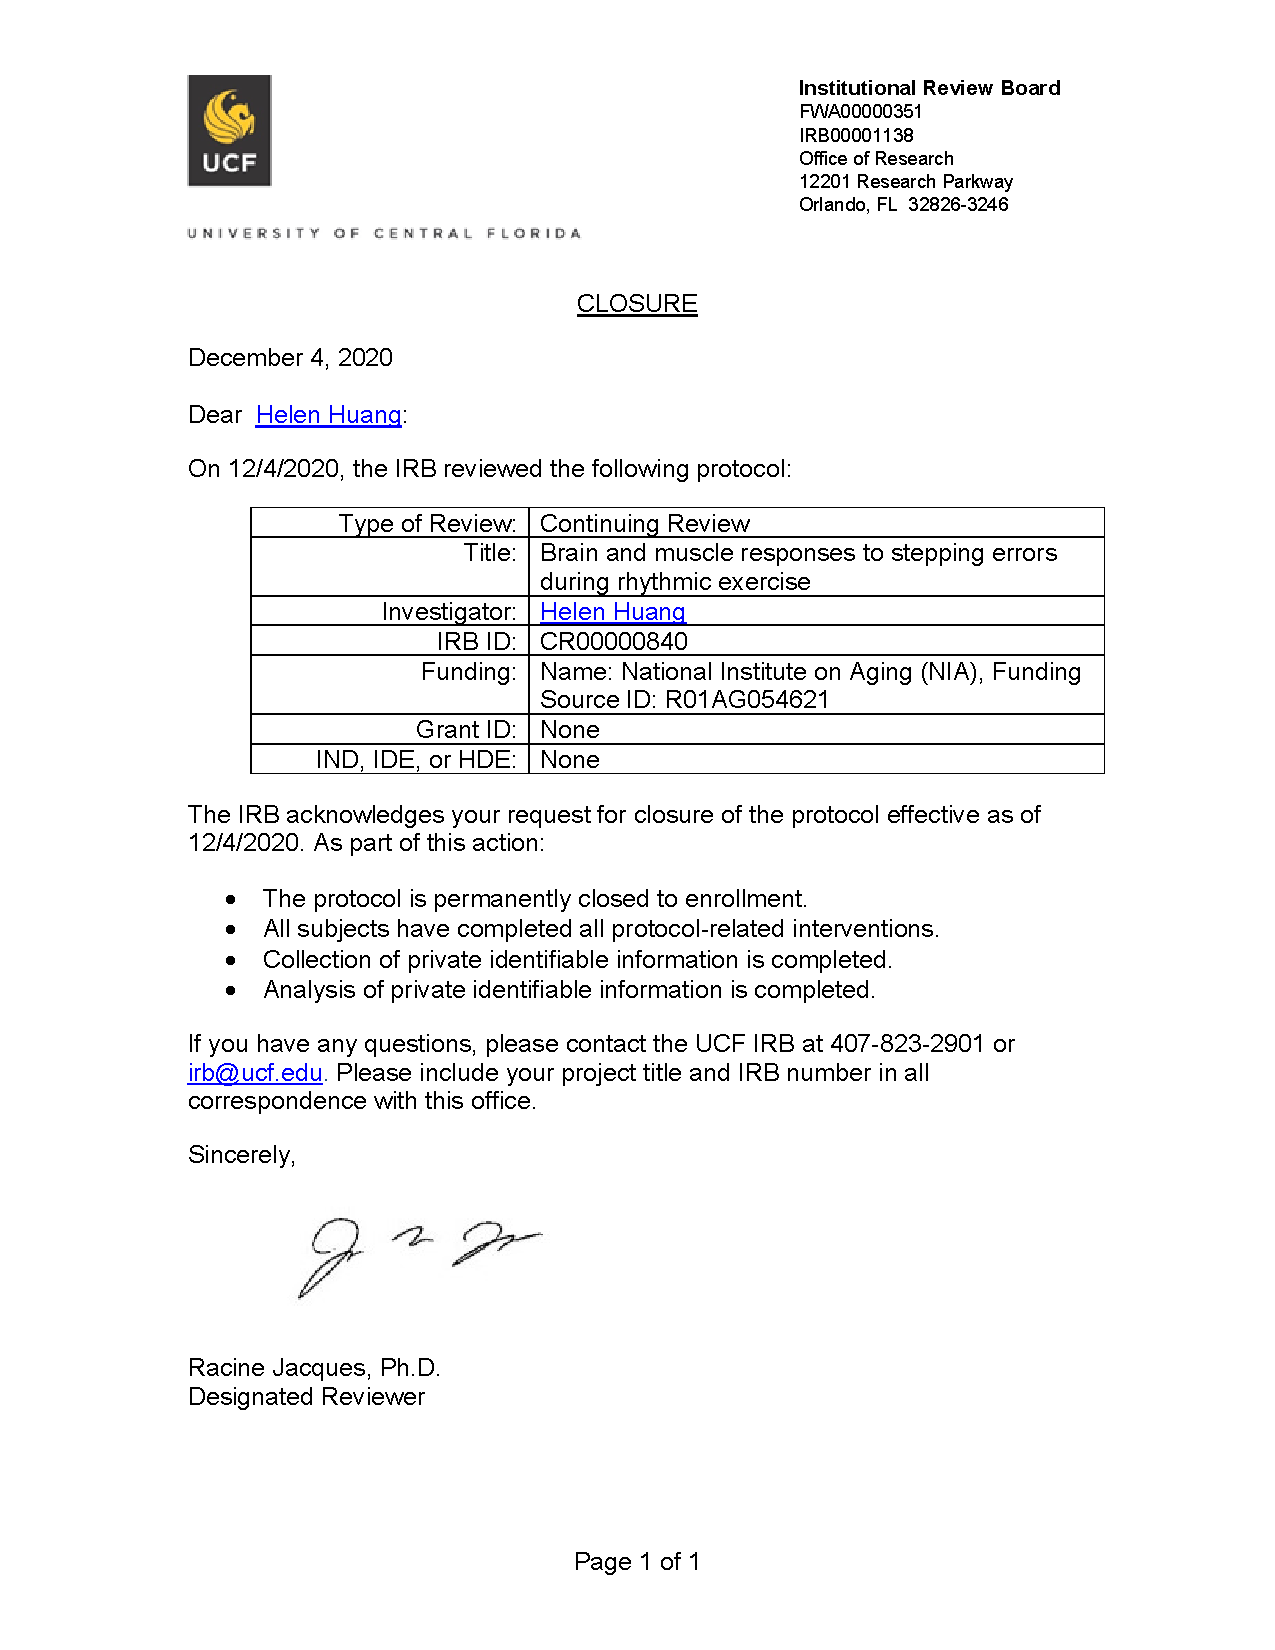
\includepdf[pages=-,scale=.8,pagecommand={}]{img/IRB approval and closure.pdf}


\chapter{COPYRIGHT PERMISSION LETTERS}
\newpage
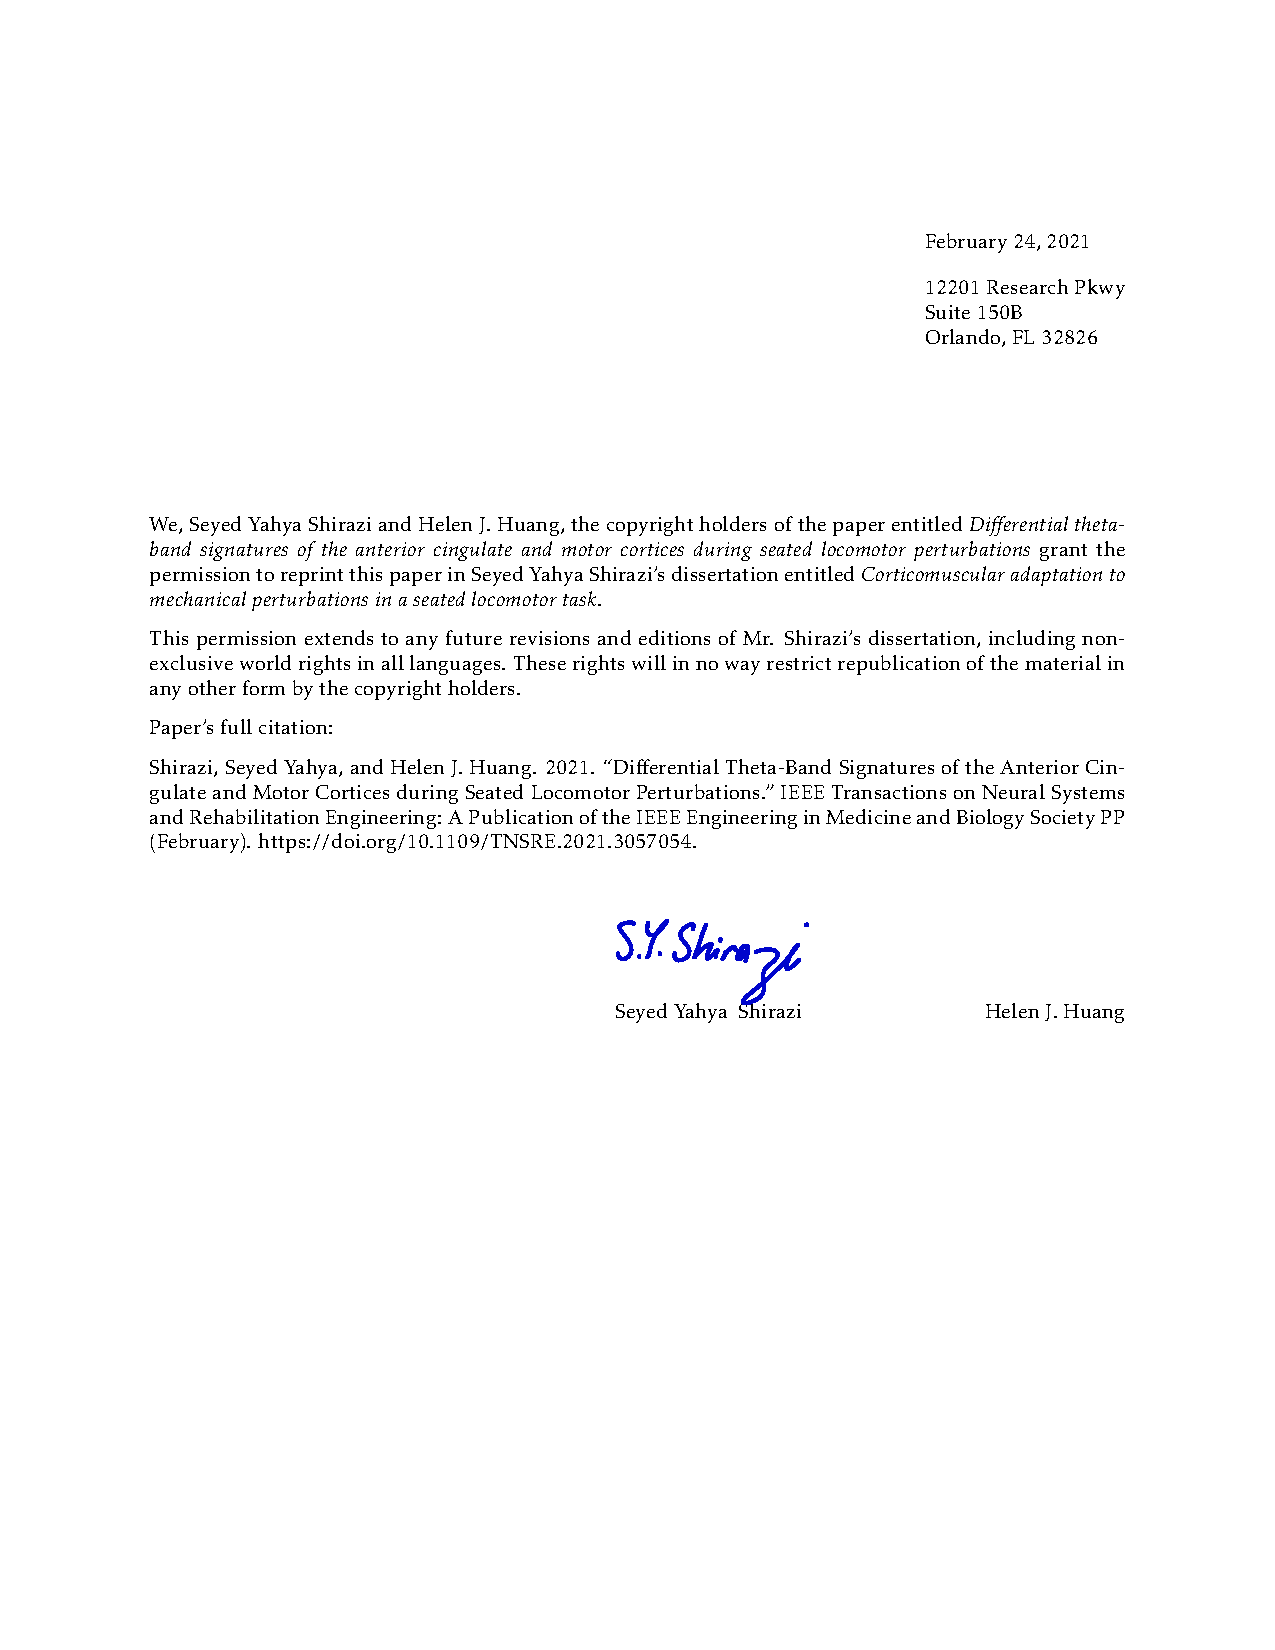
\includepdf[pages=-,scale=.8,pagecommand={}]{img/copyright authorization letters_signed-seyed.pdf}

\backmatter


\end{document}